%% Template for ENG 401 reports
%% by Robin Turner
%% Adapted from the IEEE peer review template

%
% note that the "draftcls" or "draftclsnofoot", not "draft", option
% should be used if it is desired that the figures are to be displayed in
% draft mode.

\documentclass[peerreview]{IEEEtran}
\usepackage{cite} % Tidies up citation numbers.
\usepackage{url} % Provides better formatting of URLs.
\usepackage[utf8]{inputenc} % Allows Turkish characters.
\usepackage{booktabs} % Allows the use of \toprule, \midrule and \bottomrule in tables for horizontal lines
\usepackage{graphicx}


\hyphenation{op-tical net-works semi-conduc-tor} % Corrects some bad hyphenation 



\begin{document}
%\begin{titlepage}
% paper title
% can use linebreaks \\ within to get better formatting as desired
\title{Balloma Video Game playing Reinforcement Learning Agent.}


% author names and affiliations

\author{Luis Rojas Aguilera \\
Udacity\\
Capstone Project Proposal\\
}
\date{25/4/15}

% make the title area
\maketitle
\tableofcontents
\listoffigures
\listoftables
%\end{titlepage}

\IEEEpeerreviewmaketitle
\begin{abstract}
The abstract does not only mention the paper, but is the original paper shrunken to approximately 200 words. It states the purpose, reports the information obtained, gives conclusions, and recommendations. In short, it summarizes the main points of the study adequately and accurately. It provides information from every major section in the body of the report in a dense and compact way. Past tense and active voice is appropriate when describing what was done. If there is any, it includes key statistical detail.  

Depending on the format you use, the abstract may come on the title page or at the beginning of the main report.

\end{abstract}





\section{Introduction}
This will be a revised version of the introduction in your proposal.

\section{Problem Definition}
This will be a revised version of the problem definition in your proposal.


% An example of a floating figure using the graphicx package.
% Note that \label must occur AFTER (or within) \caption.
% For figures, \caption should occur after the \includegraphics.
% Note that IEEEtran v1.7 and later has special internal code that
% is designed to preserve the operation of \label within \caption
% even when the captionsoff option is in effect. However, because
% of issues like this, it may be the safest practice to put all your
% \label just after \caption rather than within \caption{}.
%
% Reminder: the "draftcls" or "draftclsnofoot", not "draft", class
% option should be used if it is desired that the figures are to be
% displayed while in draft mode.
%
\begin{figure}[!h]
\centering
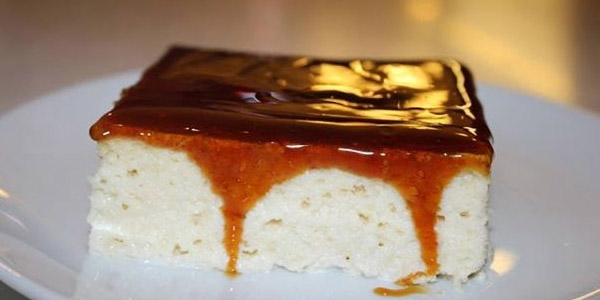
\includegraphics[width=0.8\columnwidth]{trilece} 
\caption{Simulation Results}
\label{fig_sim}
\end{figure}

% Note that IEEE typically puts floats only at the top, even when this
% results in a large percentage of a column being occupied by floats.

\section{Proposed Solutions}
This may be a modified version of your proposal depending on previously carried out research or any feedback received.  
\subsection{Your first solution}
Describe your first solution here.
\subsection{Your second solution}
Describe your second solution here.
\subsection{Your third solution}
Describe your third solution here.
\subsubsection{Subsubsection Heading Here}
Use the subsubsection command with caution---you probably won't need it at, but I'm including it this an example.

\section{Criteria for Assessing Solutions} \label{sec:criteria}
This may be a modified version of your proposal depending on previously carried out research or any feedback received.  



\section{Research Methodology}
The main difference between this section and the one in your report proposal is use of verb tense: there you suggested what you will do and here you will describe what you did. Be concise and precise when outlining how you researched your potential solutions. 
Remember that your research should be guided by: 
\begin{itemize}
\item Relevance to the context of application  
\item Your assessment criteria 
\item Practicality 
\end{itemize}
So it may be worth commenting on your research methodology in light of the above (e.g., justifying a particular approach).  

In this section, only describe how you collected data, and explain what you did to test your criteria.  \emph{Do not include your findings in this section.}

\section{Analysis and Interpretation}
 In this section you will mainly analyze your data in terms of your assessment criteria; e.g., do the data suggest that a particular solution is ``cost effective'' ``environmentally acceptable'', ``technically feasible'' or ``affordable''?
   
Be logical and selective when analyzing/interpreting your research data.  For example, if a proposed solution is proven to be far too expensive to realistically implement in your context, is there any value in discussing whether it is ``culturally viable'' or ``technically sustainable''? Perhaps in this case you can focus more attention on solutions that your research suggests are more valid.  Do not just throw huge quantities of raw data at your reader and leave them to interpret it. Present enough to transparently support any conclusions you draw and make sure that you offer justifications for your analysis.  

Be honest and reflective while discussing your data. Your data might be too limited or unclear to interpret with accuracy---explain this, perhaps suggesting how this shortcoming could be addressed. Admitting the above will help you draw more honest and worthwhile conclusions.  

Remember that research is an imperfect and ongoing process that should be open to question and verification. Therefore, unless convinced by the absolute strength of your evidence, you should be tentative in your language choice when interpreting/analyzing research results. Selectively use {\em hedging} (language which indicates a lack of certainty) to modify the tone of your analysis and any conclusions that result from this. 

Here are some examples that show differing degrees of certainty:
\begin{itemize}  
\item it appears that \ldots
\item it can be tentatively concluded that \ldots
\item it is almost certain that \ldots
\item perhaps the evidence indicates \ldots
\item this seems to point to the fact that \ldots
\item this could be interpreted as evidence of \ldots
\item without doubt its application would prove beneficial for \ldots
\end{itemize}

Finally, don’t introduce any new content (e.g., research methods or solutions) within this section---this will prove confusing for the reader. The reader should clearly understand that you are, based on specific criteria, interpreting the results of your research in order to test the viability of various solutions to remedy a particular problem. The sole function of this part of the report is to openly discuss your research findings in order to set up your conclusions/recommendations.


% Example of a table from http://www.latextemplates.com/template/professional-table
\begin{table} % Add the following just after the closing bracket on this line to specify a position for the table on the page: [h], [t], [b] or [p] - these mean: here, top, bottom and on a separate page, respectively
\centering % Centers the table on the page, comment out to left-justify
\begin{tabular}{l c c c c c} % The final bracket specifies the number of columns in the table along with left and right borders which are specified using vertical bars (|); each column can be left, right or center-justified using l, r or c. To specify a precise width, use p{width}, e.g. p{5cm}
\toprule % Top horizontal line
& \multicolumn{5}{c}{Growth Media} \\ % Amalgamating several columns into one cell is done using the \multicolumn command as seen on this line
\cmidrule(l){2-6} % Horizontal line spanning less than the full width of the table - you can add (r) or (l) just before the opening curly bracket to shorten the rule on the left or right side
Strain & 1 & 2 & 3 & 4 & 5\\ % Column names row
\midrule % In-table horizontal line
GDS1002 & 0.962 & 0.821 & 0.356 & 0.682 & 0.801\\ % Content row 1
NWN652 & 0.981 & 0.891 & 0.527 & 0.574 & 0.984\\ % Content row 2
PPD234 & 0.915 & 0.936 & 0.491 & 0.276 & 0.965\\ % Content row 3
JSB126 & 0.828 & 0.827 & 0.528 & 0.518 & 0.926\\ % Content row 4
JSB724 & 0.916 & 0.933 & 0.482 & 0.644 & 0.937\\ % Content row 5
\midrule % In-table horizontal line
\midrule % In-table horizontal line
Average Rate & 0.920 & 0.882 & 0.477 & 0.539 & 0.923\\ % Summary/total row
\bottomrule % Bottom horizontal line
\end{tabular}
\smallskip 
\caption{Some impressive numbers} % Table caption, can be commented out if no caption is required
\label{tab:template} % A label for referencing this table elsewhere, references are used in text as \ref{label}
\end{table}
A reference to Table \ref{tab:template}.

\section{Conclusions and Recommendations}
Conclusion shows what knowledge comes out of the report. As you draw a conclusion, you need to explain it in terms of the preceding discussion. You are expected to repeat the most important ideas you have presented, without copying. Adding a table/chart summarizing the results of your findings might be helpful for the reader to clearly see the most optimum solution(s). 

It is likely that you will briefly describe the comparative effectiveness and suitability of your proposed solutions. Your description will logically recycle language used in your assessing criteria (section \ref{sec:criteria}): ``Solution A proved to be the most cost effective of the alternatives'' or ``Solution B, though a viable option in other contexts, was shown to lack adaptability''.  Do not have detailed analysis or lengthy discussions in this section, as this should have been completed in section X. 
 
As for recommendations, you need to explain what actions the report calls for. These recommendations should be honest, logical and practical. You may suggest that one, a combination, all or none of your proposed solutions should be implemented in order to address your specific problem. You could also urge others to research the issue further, propose a plan of action or simply admit that the problem is either insoluble or has a low priority in its present state.   

The recommendations should be clearly connected to the results of the report, and they should be explicitly presented. Your audience should not have to guess at what you intend to say.  




\appendices
\section{What Goes in the Appendices} \label{App:WhatGoes}
The appendix is for material that readers only need to know if they are studying the report in depth. Relevant charts, big tables of data, large maps, graphs, etc. that were part of the research, but would distract the flow of the report should be given in the Appendices. 
\section{Formatting the Appendices} \label{App:Formatting}
Each appendix needs to be given a letter (A, B, C, etc.) and a title. \LaTeX will do the lettering automatically.


\begin{thebibliography}{1}
% Here are a few examples of different citations 
% Book
\bibitem{kopka_1999} % Note the label in the curly brackets. Use the cite the source; e.g., \cite{kopka_latex}
H.~Kopka and P.~W. Daly, \emph{A Guide to \LaTeX}, 3rd~ed.\hskip 1em plus
  0.5em minus 0.4em\relax Harlow, England: Addison-Wesley, 1999.
\bibitem{horowitz_2005}D.~Horowitz, \emph{End of Time}. New York, NY, USA: Encounter Books, 2005. [E-book] Available: ebrary, \url{http://site.ebrary.com/lib/sait/Doc?id=10080005}. Accessed on: Oct. 8, 2008.
% Article from database
\bibitem{castlevecchi_2008}D.~Castelvecchi, ``Nanoparticles Conspire with Free Radicals'' \emph{Science News}, vol.174, no. 6, p. 9, September 13, 2008. [Full Text]. Available: Proquest, \url{http://proquest.umi.com/pqdweb?index=52&did=1557231641&SrchMode=1&sid=3&Fmt=3&VInst=PROD&VType=PQD&RQT=309&VName=PQD&TS=1229451226&clientId=533}. Accessed on: Aug.~3, 2014.
% Conference Paper from the Internet
\bibitem{lach_2010}J.~Lach, ``SBFS: Steganography based file system,'' in \emph{Proceedings of the 2008 1st International Conference on Information Technology, IT 2008, 19-21 May 2008, Gdansk, Poland.} Available: IEEE Xplore, \url{http://www.ieee.org}. [Accessed: 10 Sept. 2010].
% Web page, no author
\bibitem{a_laymans_explanation}``A `layman's' explanation of Ultra Narrow Band technology,'' Oct.~3, 2003. [Online]. Available: \url{http://www.vmsk.org/Layman.pdf}. [Accessed: Dec.~3, 2003]. 
\end{thebibliography}

% This is a hand-made bibliography. If you want to use a BibTeX file, you're on your own ;-)














\end{document}


